\documentclass[../tp3_grupo404.tex]{subfiles}

\graphicspath{{\subfix{../out/}}}

\begin{document}

Para probar que el problema \textquote{set dominante} es \emph{NP-Completo} tenemos que probar que el problema
sea \emph{NP} y también \emph{NP-Hard}.

\textbf{1. Set dominante es NP}: Dado un set puedo recorrer cada vértice, marcarlo junto con
sus vértices adyacentes y comprobar que todos los vértices del grafo fueron marcados.
Un algoritmo que certifica el problema podría ser:

\begin{alternate}[breaklines=true,numbers=left,xleftmargin=5mm]
    def es_set_dominante(grafo, set):
    visitados = []
    for vertices in set:
        if vertice not in visitados:
            visitados.append(vertice)
        for v_adyacente in vertice:
            if v_adyacente not in visitados:
                visitados.append(v_adyacente)
    if len(visitados) == len(grafo):
        return true
    return false
\end{alternate}

Su complejidad es de$ O(n2)$ y por lo tanto puedo decir que es un certificador eficiente.
Luego, puedo decir que el problema de set dominante es \emph{NP}.

\textbf{2. Set dominante es NP-Hard}: Para demostrar que el problema del conjunto dominante es \emph{NP-Hard}, 
necesitamos mostrar que un problema conocido \emph{NP-Completo} es reducible en tiempo polinómico a un problema de 
conjunto dominante. En este caso elegimos el problema de cobertura de vértices (\emph{vertex cover}) como 
problema \emph{NP-Completo} conocido.

La cobertura de vértices en un grafo no dirigido $G(V,E)$ es un subconjunto de vértices $V'$ de $V$, tal 
que cada arista en el grafo $G$ está conectada con al menos un vértice de $V'$. Este problema entonces 
busca si existe una cobertura de vértices de un tamaño dado k para un grafo no dirigido dado $G(V,E)$.

Los dos problemas parecen ser bastante similares, pero hay una diferencia esencial, que se da en el caso 
que el grafo tenga vértices aislados. En el caso de \emph{vertex cover} estos vértices pueden ignorarse ya que 
no hay ninguna arista conectada a ellos. En cambio, en el caso del \emph{set dominante}, esos vértices deberían 
incluirse en el conjunto dominante, ya que no hay ningún vértice adyacente a ellos.

Queremos demostrar que dada una instancia de un problema de \emph{vertex cover} $(G,k)$, podemos producir una 
instancia equivalente de un problema \emph{set dominante} en tiempo polinómico.
Para reducir del problema de \emph{vertex cover} al de \emph{set dominante}, necesitamos construir un nuevo grafo $G'$ 
desde el grafo $G$ dado. Al inicio, $G'$ es un duplicado de $G$. Luego, por cada arista ${u,v}$ en $G$ creamos un 
nuevo vértice $w_{uv}$ en $G'$ y agregamos aristas ${u, w}$ y ${v, w}$ en $G'$. Sea $n_{a}$ el número de 
vértices aislados y $k' = k + n_{a}$. Esta reducción se muestra en la figura siguiente.

\begin{figure}[H]
    \centering
    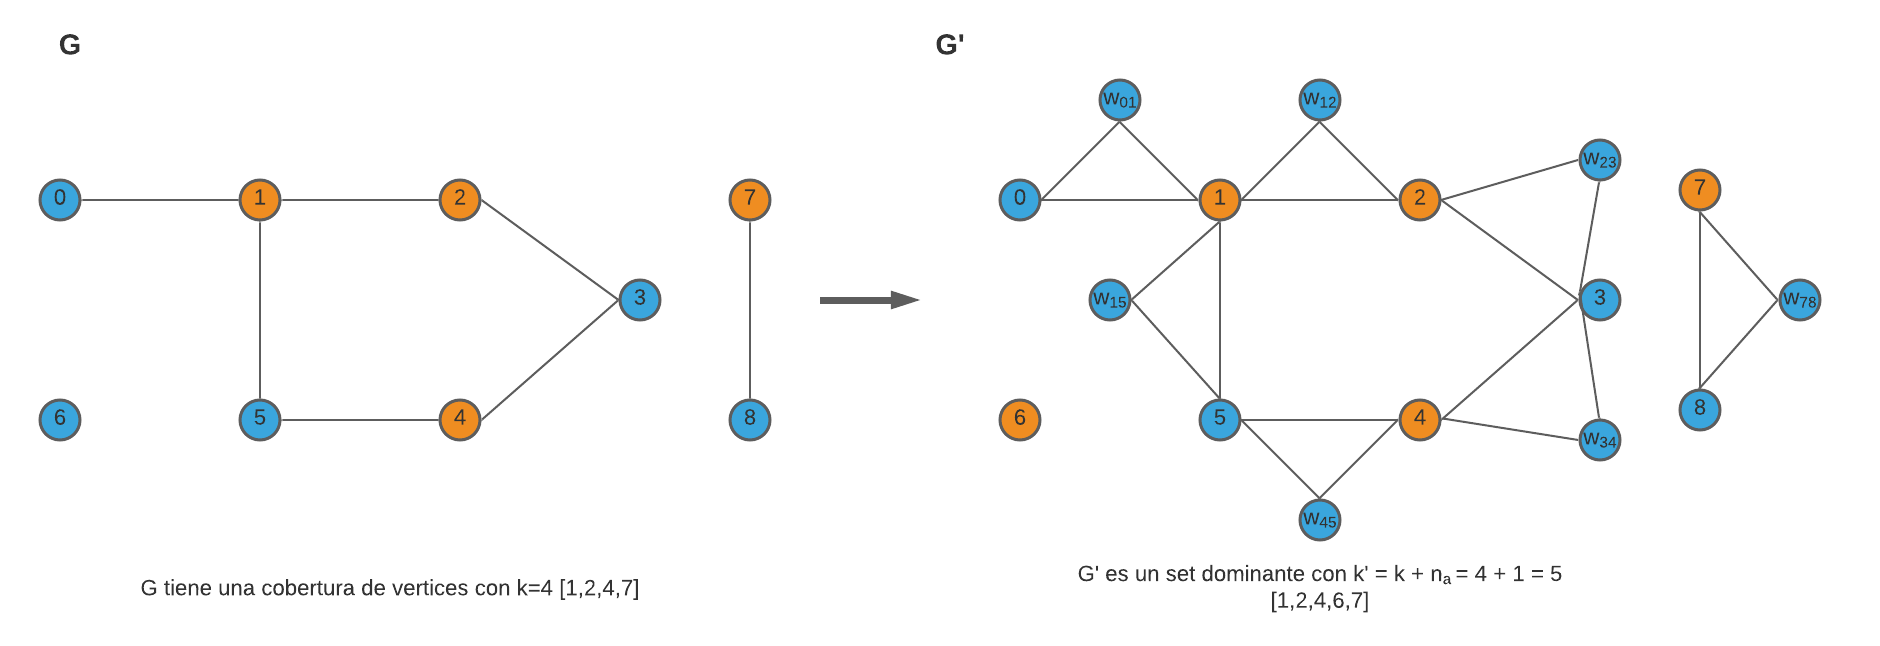
\includegraphics[width=0.9\linewidth,angle=0,origin=c]{out/vertex_to_dominant.png}
\end{figure}

\begin{alternate}[breaklines=true,numbers=left,xleftmargin=5mm]
    def es_set_dominante(grafo, set):
    visitados = []
    for vertice in set:
        if vertice not in visitados:
            visitados.append(vertice)
        for v_adyacente in vertice:
            if v_adyacente not in visitados:
                visitados.append(v_adyacente)
    if len(visitados) = len(grafo):
        return true
    return false
\end{alternate}

La reducción tiene complejidad $O(V+E)$ y por lo tanto se puede reducir polinomialmente.
Para establecer la correctitud de la reducción necesitamos demostrar que un grafo $G$ tiene una cobertura 
de vértices de tamaño $k$ si y sólo si $G'$ tiene un set dominante de tamaño $k'$.

=>) Como primera medida chequeamos que si $V'$ es una cobertura de vértices de $G$, entonces $V''=V' U V_{a}$ es un 
set dominante para $G'$ donde $V_{a}$ son los vértices aislados.
Para observar si $V''$ es un set dominante, primero observemos que todos los vértices aislados son parte de $V''$. 
Luego, todos los vértices agregados $w_{uv}$ en $G'$ corresponden a una arista ${u,v}$ en $G$, implicando que $u$ o $v$ 
pertenecen a la cobertura de vértices $V'$. Por ende, $w_{uv}$ va a estar dominado por el mismo vértice en $V''$. 
Finalmente, cada uno de los vértices no aislados originales, va a estar conectado al menos a una arista, 
y por consiguiente va a ser parte de $V'$ o por el contrario todos sus vecinos van a ser parte de $V'$. 
Entonces, cada vértice no aislado original está en $V''$ o es adyacente a un vértice en $V''$.

<=) Ahora queremos demostrar que si $G'$ tiene un set dominante $V''$ de tamaño $k'=k+n_{a}$, entonces $G$ tiene una 
cobertura de vértices $V'$ de tamaño $k$. Todos los vértices aislados de $G'$ deben ser parte del set dominante. 
Sea $V'''$ los vértices pertenecientes al set dominante $V''$ que no son aislados, algunos de estos vértices van 
a ser de los que fueron especialmente creados y que no son parte del grafo original $G$. Podemos afirmar que 
no es necesario utilizar ninguno de estos vértices creados en $V'''$, ya que si algún vértice nuevo $w_{uv}$ 
(que es adyacente solo a los vértices originales $u$ y $v$) pertenece a $V'''$, entonces podemos modificar 
$V'''$ reemplazando $w_{uv}$ por $u$ o $v$. Suponiendo que lo reemplazamos por $u$, $u$ seguirá dominando a $v$ y $w$. 
Por ende reemplazando $w$ con $u$ en el set dominante, se siguen dominando los mismos vértices, y potencialmente 
incluso alguno más. Denotemos como $V'$ el set dominante luego de esta modificación.

\begin{figure}[H]
    \centering
    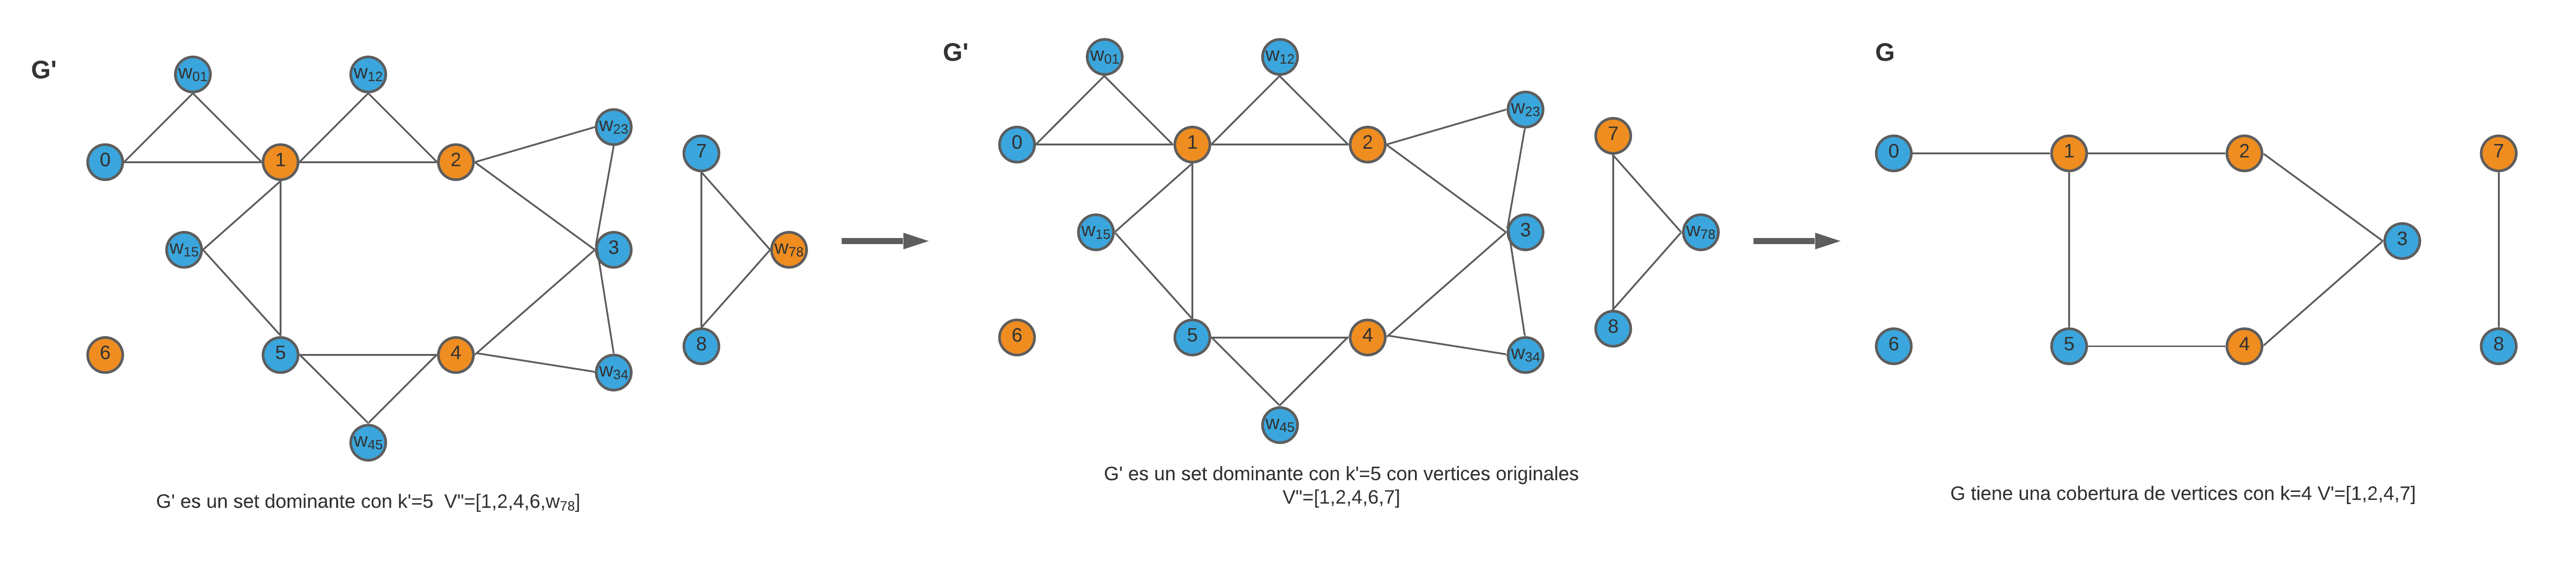
\includegraphics[width=0.9\linewidth,angle=0,origin=c]{out/dominant_to_vertex.png}
\end{figure}

Finalmente, podemos afirmar que $V'$ es una cobertura de vértices para $G$. Si por el contrario, 
existiese alguna arista ${u,v}$ de $G$ que no estuviese cubierta, es decir, que $u$ o $v$ no estuviesen 
en $V'$, entonces los vértices creados $w_{uv}$ no serían adyacente a ningún vértice de $V''$ en $G'$, 
contradiciendo la hipótesis de que $V''$ era un set dominante para $G'$.
Por ende, podemos concluir que el problema del set dominante es un problema \emph{NP-Completo}.


% FIN DEL DOCUMENTO (SECCIÓN Reentrega P2.2)
% NO BORRAR POR ACCIDENTE NI ESCRIBIR COSAS ABAJO
\end{document}